\section{Theoretical thresholds via Rademacher complexity}\label{sec::rademacher}
% \textcolor{blue}{
% Analysis with the Rademacher complexity and the "theoretical threshold". Need for a low sample complexity, such as with HIPM, whereas WoW would give bad results. Show an example where the theoretical threshold is good (e.g. number of observations is $n$ high, two Dirichlet processes with different concentration) and one that is not good (e.g. two dirichlet processes with similar base measure, e.g. uniform and beta, or parametric model of panaretos). Insist that it is a bound that holds uniformly on the infinitely dimensional set of distributions, and thus is conservative.}


% polished start
This section develops a uniform, nonparametric threshold for hypothesis testing derived from Rademacher complexity. The primary objective is to establish a concentration inequality for the distance between two hierarchical estimators. Intuitively, given two laws of random probability measures $Q^1, Q^2$, whether the distance function $d$ is WoW or HIPM, $d(Q^1_{n,m}, Q^2_{n,m})$ should be close to $d(Q^1, Q^2)$. A concentration inequality quantifies how close these quantities are for a given probability level. In particular, for $\theta \in (0,1)$, it provides a radius $r(n, m, \theta)$, depending on $n, m$, and $\theta$, such that the probability that $d(Q^1_{n,m}, Q^2_{n,m})$ is within radius $r(n, m, \theta)$ of $d(Q^1, Q^2)$ is at least $1 - \theta$. This implies that under the null hypothesis, for every $\theta \in (0, 1)$, $d(Q^1_{n,m}, Q^2_{n,m})$ will be smaller than the $r(n, m, \theta)$ with probability at least $1 - \theta$. Therefore, if we use $r(n, m, \theta)$ as a threshold function and reject $H_0$ whenever 
\[
d(Q^1_{n,m}, Q^2_{n,m}) > r(n, m, \theta),
\]
we are guaranteed that the probability of making a Type I error is at most $\theta$. Let us now discuss how to obtain the threshold function $r(n, m, \theta)$ and its relationship to the Rademacher complexity of the function class that defines the distance function.

The main tool for obtaining such a result is Talagrand’s inequality (see Proposition B.1 in \cite{sriperumbudur2012empirical}). The radius function, as described above, is provided for a random variable of a specific form, which includes integral probability metrics. The dominant term in the radius function is the expected value of the random variable of interest. Following standard symmetrization arguments from empirical process theory, we bound this expectation using the Rademacher complexity of the underlying function class. This approach yields the following theoretical results:
\begin{theorem}[Threshold for HIPM] \label{theorem::radem_threshold_hipm}
Let $\X$ be a compact subset of $\R^d$, and let $Q^1, Q^2 \in \probprobx$. Then, there exists a function $r_d(n, m, \theta)$ such that for all $n, m \geq 1$ and $\theta \in (0,1)$,
\[
\mathbb{P}\left( \left| \dlip(Q^1_{n,m}, Q^2_{n,m}) - \dlip(Q^1, Q^2) \right| \geq r_d(n,m,\theta) \right) \leq \theta,
\]
where for a fixed $\theta$,
\[
r_d(n, m, \theta) = 
\begin{cases}
    \mathcal{O} \left( \frac{1}{\sqrt{n}} + \frac{1}{\sqrt{m}}\right), & \text{if } d = 1 \\
    \mathcal{O} \left( \frac{1}{\sqrt{n}}\log(n) + \frac{1}{\sqrt{m}}\log(m)\right), & \text{if } d = 2 \\
    \mathcal{O} \left( \frac{1}{n^{\frac{1}{d}}} + \frac{1}{m^{\frac{1}{d}}}\right), & \text{if } d > 2.
\end{cases}
\]
\end{theorem}
A similar theorem is obtained for the Wasserstein over Wasserstein distance. 
\begin{theorem}[Threshold for WoW]
\label{theorem::radem_threshold_wow}
Let $\X$ be a compact subset of $\R^d$, and let $Q^1, Q^2 \in \probprobx$. Then, there exists an integer $N \geq 1$ and a function $r_d(n, m, \theta)$ such that for all $n \geq N$, $m \geq 1$, and $\theta \in (0, 1)$,
\[
\mathbb{P}\left( \left| \WW(Q^1_{n,m}, Q^2_{n,m}) - \WW(Q^1, Q^2)\right| \geq r_d(n, m, \theta) \right) \leq \theta,
\]
where for a fixed $\theta$,
\[
r_d(n, m, \theta) = 
\begin{cases}
    \mathcal{O} \left(\frac{\log(\log(n))}{\log(n)} + \frac{1}{\sqrt{n}} + \frac{1}{\sqrt{m}}\right), & \text{if } d = 1 \\
    \mathcal{O} \left(\frac{\log(\log(n))}{\log(n)} + \frac{1}{\sqrt{n}}\log(n) + \frac{1}{\sqrt{m}}\log(m)\right), & \text{if } d = 2 \\
    \mathcal{O} \left(\frac{\log(\log(n))}{\log(n)} + \frac{1}{n^{\frac{1}{d}}} + \frac{1}{m^{\frac{1}{d}}}\right), & \text{if } d > 2.
\end{cases}
\]
\end{theorem}
\begin{remark}
If $\X = [a,b]$, the exact form of the threshold function in Theorem \ref{theorem::radem_threshold_hipm} can be derived, as the bound for the Rademacher complexity is known in closed form. In this case, we obtain a finite-sample guarantee for the Type I error. Note that for the WoW distance, even if the exact threshold were known, the finite-sample guarantee would hold only for $n \geq N$ for some integer $N \geq 1$. 
\end{remark}

\begin{remark}
    Theorems \ref{theorem::radem_threshold_hipm} and \ref{theorem::radem_threshold_wow} can be extended to more general spaces $\X$, provided that one can bound the Rademacher complexity of the function class over which the IPM is defined. Whether an exact threshold can be obtained depends on whether the bound on the Rademacher complexity is exact or merely an asymptotic upper bound.
\end{remark}
The consequence of the theorems above is a testing scheme which, given a significance level $\theta$, rejects the null hypothesis whenever the observed distance between the hierarchical estimators exceeds the threshold from the aforementioned theorems. In addition to controlling the Type I error, these theorems also ensure consistency. Intuitively, under $H_1$, the observed distance $d(Q^1_{n,m}, Q^2_{n,m})$, whether $d$ is WoW or HIPM, will be close to $d(Q^1, Q^2)$. Hence, as long as the threshold $r_d(n, m, \theta)$ converges to $0$ as $n, m \to \infty$, we will eventually have $d(Q^1_{n,m}, Q^2_{n,m}) > r_d(n, m, \theta)$. The theorems below formalize this intuition. Note that in the limits below, there is no dependency between $n$ and $m$ in how they converge to infinity.

\begin{theorem}[Consistency for HIPM]
\label{theorem::radem_consistency_hipm}
Let $\X$ be a compact subset of $\R^d$, and let $Q^1, Q^2 \in \probprobx$. Let $\theta$ denote the significance level, and let $r_d(n, m, \theta)$ be the threshold function from Theorem \ref{theorem::radem_threshold_hipm}. Then:
\begin{itemize}
    \item Type I error: If $Q^1 = Q^2$, then  
    $$\mathbb{P}\left( \dlip(Q_{n,m}^1, Q_{n,m}^2) > r_d(n,m, \theta) \right) \leq \theta \quad \text{for all } n, m \geq 1.$$
    \item Consistency: If $Q^1 \neq Q^2$, then  
    $$\lim_{n,m\to \infty}\mathbb{P}\left( \dlip(Q_{n,m}^1, Q_{n,m}^2) > r_d(n,m, \theta) \right) = 1.$$
\end{itemize}
\end{theorem}

\begin{theorem}[Consistency for WoW]
\label{theorem::radem_consistency_wow}
Let $\X$ be a compact subset of $\R^d$, and let $Q^1, Q^2 \in \probprobx$. Let $\theta$ denote the significance level, and let $r_d(n, m, \theta)$ be the threshold function from Theorem \ref{theorem::radem_threshold_wow}. Then, there exists $N \geq 1$ such that:
\begin{itemize}
    \item Type I error: If $Q^1 = Q^2$, then  
    $$\mathbb{P}\left( \WW(Q_{n,m}^1, Q_{n,m}^2) > r_d(n,m, \theta) \right) \leq \theta \quad \text{for all } n \geq N, m \geq 1.$$
    \item Consistency: If $Q^1 \neq Q^2$, then  
    $$\lim_{n,m\to \infty}\mathbb{P}\left( \WW(Q_{n,m}^1, Q_{n,m}^2) > r_d(n,m, \theta) \right) = 1.$$
\end{itemize}
\end{theorem}
While theoretically appealing, the aforementioned theorems have practical limitations. Achieving high power requires the threshold to decay to zero at a sufficiently fast rate. However, the logarithmic terms present in the threshold for the WoW distance result in a threshold function that converges to zero at a suboptimal rate. Furthermore, although using the HIPM provides a parametric rate, the magnitude of the constant term within the function often makes the testing scheme impractical for finite samples.

These limitations are demonstrated by our numerical simulations. We restrict our simulations to the HIPM, as the threshold associated with the WoW distance is even more conservative than that of the HIPM. 

Suppose that we have two different laws of RPMs, $Q^1, Q^2 \in \probprobx$. For a fixed probability level $\theta \in (0,1)$, to obtain a low Type II error, the theoretical threshold should be less than the empirical threshold. The empirical threshold is defined as the $(1-\theta)$-quantile of the random variable $\dlip(Q_{n,m}^1, Q_{n,m}^2)$. In the figure below, we display how the theoretical and empirical thresholds differ for a fixed $\theta$ as $n$ and $m$ increase.

Fix $\theta = 0.15$ and consider two Dirichlet processes $Q^1 = \text{DP}(1.0, P_0)$ and $Q^2 = \text{DP}(1.5, P_0)$, where $P_0 = \operatorname{Law}(Z)$ and
\[
Z = \begin{cases}
0.25X - 1, & \text{with probability } 0.5, \\[6pt]
0.25X + 0.75, & \text{with probability } 0.5,
\end{cases}
\]
with $X \sim \text{Unif}(0,1)$.

As shown in Figure \ref{fig:radem_threshold_plots}, the theoretical threshold is significantly larger than the empirical threshold, even for large values of $n$ and $m$. Consequently, the null hypothesis is never rejected when it is false. The reason for such a large theoretical threshold is that it is designed to be uniform over the entire space of laws of random probability measures.

\begin{figure}[H]
    \centering
    \begin{subfigure}{0.32\textwidth}
        \centering
        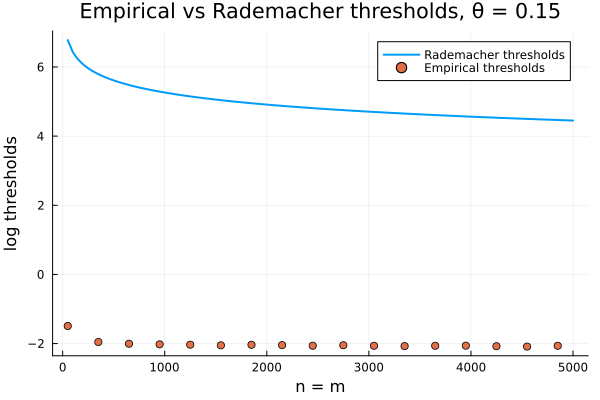
\includegraphics[width = \linewidth]{chapters/two-sample-testing/figures/ch4/emp_radem_plot_fixed_theta.png}
    \end{subfigure}
    \begin{subfigure}{0.32\textwidth}
        \centering
        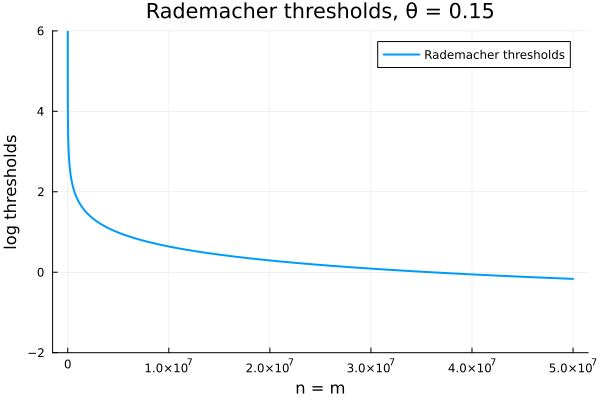
\includegraphics[width = \linewidth]{chapters/two-sample-testing/figures/ch4/radem_plot_vary_theta.png}
    \end{subfigure}
    \caption{}
    \label{fig:radem_threshold_plots}
\end{figure}

% polished end



% This section develops a uniform, nonparametric threshold for hypothesis testing derived from Rademacher complexity. The primary objective is to establish a concentration inequality for the distance between two hierarchical estimators. Intuitively, given two laws of random probability measure $Q_1, Q_2,$ whether the distance function $d$ is WoW or HIPM, $d\left(Q^1_{n,m}, Q^2_{n,m} \right)$ should be close to $d\left(Q^1, Q^2\right).$ Concentration inequality quantifies how close it will be for a given probability level. In particular, for $\theta \in (0,1)$, it gives us the radius $r(n, m, \theta)$ depending on $n, m$ and $\theta$ such that probability that $d\left(Q^1_{n,m}, Q^2_{n,m} \right)$ is within $r(n, m, \theta)$ radius from $d\left(Q^1, Q^2\right)$ is higher than $1 - \theta.$ This implies that under the null hypothesis, for every $\theta \in (0, 1),$ we know that $d\left(Q^1_{n,m}, Q^2_{n,m} \right)$ will be smaller than radius $r(n, m, \theta)$ with probability at least $1 - \theta.$ So, if we use $r(n, m, \theta)$ as a threshold function, and reject $H_0$ whenever 
% \[
% d\left(Q^1_{n,m}, Q^2_{n,m} \right) > r(n, m, \theta),
% \]
% we are guaranteed that the probability of making a Type I error is at most $\theta.$ Let us now discuss how to obtain the threshold function $r(n, m, \theta)$ and how it is related to the Rademacher complexity of the function class which defines the distance function.

% The main tool for obtaining such a result is Talagrand’s inequality (see Proposition B.1 in \cite{sriperumbudur2012empirical}). The radius function, as described above, is provided for a random variable that has a specific form, which also includes integral probability metrics. The dominant term in the radius function is the expected value of the random variable of interest. Following standard symmetrization arguments from empirical process theory, we bound this expectation using the Rademacher complexity of the underlying function class. This approach yields the following theoretical results:








% Recall that our focus is on the nonparametric setting, meaning that we do not make any assumptions on the laws of random probability measures. Given two such laws, $Q^1, Q^2 \in \probprobx$, we observe hierarchical samples from which we compute the distance between hierarchical estimators, $d(Q^1_{n,m}, Q^2_{n,m})$. In this section, we study testing schemes based on two distance functions: the Wasserstein-over-Wasserstein distance and the Hierarchical IPM. Recall that both of these distances are special cases of Integral Probability Metric.  

% The main idea of our testing scheme is to construct a rejection region such that the probability of observing a random variable falling into this region under the null hypothesis is small. Typically, this is achieved by comparing $d(Q^1_{n,m}, Q^2_{n,m})$ to its quantile under $H_0$. In our setting, however, the quantile is unknown. Instead, for a fixed probability level $\theta$ and sample sizes $n$ and $m$, we obtain a threshold $f(n, m, \theta)$ such that the probability of observing $d(Q^1_{n,m}, Q^2_{n,m})$ exceeding this threshold is at most $\theta$. Therefore, the corresponding rejection region takes the form $(f(n,m, \theta), \infty).$



% Although Talagrand’s theorem is quite general, in that it allows random variables taking values in abstract spaces beyond $\R^d$, we still face the challenge that we do not observe i.i.d. samples from $Q^1$ and $Q^2$. To overcome this issue, we decompose the gap
% \begin{align*}
% \left| \dlip(Q_{n,m}^1,Q_{n,m}^2) - \dlip(Q^1,Q^2) \right| 
% &\leq \left| \dlip(Q_{n,m}^1,Q_{n,m}^2) - \dlip(Q_n^1,Q_n^2) \right| \\
% &\quad + \left| \dlip(Q_n^1,Q_n^2) - \dlip(Q^1,Q^2) \right|,
% \end{align*}
% where $Q^1_n = \frac{1}{n}\sum_{i = 1}^n\delta_{\widetilde{P}^1_i}$, $Q^2_n = \frac{1}{n}\sum_{i = 1}^n\delta_{\widetilde{P}^2_i}$, and $\widetilde{P}^1_1,\ldots,\widetilde{P}^1_n\overset{\mathrm{i.i.d.}}{\sim}Q^1, \widetilde{P}^2_1,\ldots,\widetilde{P}^2_n\overset{\mathrm{i.i.d.}}{\sim}Q^2.$ 
% \par The first term in the upper bound quantifies the difference between the empirical distance derived from exchangeable sequences of random variables and the distance that would be obtained from i.i.d. samples drawn from the laws of RPMs. The second term measures the discrepancy between the empirical distance obtained from i.i.d. samples from the laws of random measures and the true distance. We decompose the gap in this way because each of the deviations can be controlled in probability. Bounding the second term in probability is studied in \cite{sriperumbudur2012empirical} for the general IPM, and the corresponding threshold depends on the Rademacher complexity of the function class over which the IPM is defined.
% in the theorem below if we just say bounded, we need the closed set. Otherwise it is not polish.
% \begin{theorem}[Threshold for HIPM] \label{theorem::radem_threshold_hipm}
% Let $\X$ be a compact subset of  $\R^d$, and $Q^1,Q^2 \in \probprobx.$ Then, there exists a function $r_d(n, m, \theta)$ such that for all $n, m \geq 1$ and $\theta \in (0,1)$
% \[
% \mathbb{P}\Big( \big|\dlip Q^1_{n,m}, Q^2_{n,m}) - \dlip Q^1, Q^2) \big| \geq r_d(n,m,\theta)\Big) \leq \theta,
% \]
% where for fixed $\theta$,
% \[
% r_d(n, m, \theta) = 
% \begin{cases}
%     O \left( \frac{1}{\sqrt{n}} + \frac{1}{\sqrt{m}}\right) ,\ & \text{if } d= 1 \\
%     O \left( \frac{1}{\sqrt{n}}\log(n) + \frac{1}{\sqrt{m}}\log(m)\right) ,\ & \text{if } d = 2 \\
%     O \left( \frac{1}{n^{\frac{1}{d}}} + \frac{1}{m^{\frac{1}{d}}}\right) ,\ & \text{if } d > 2
% \end{cases}
% \]







% \label{theorem::radem_threshold_hipm}
% Given $\X = [a,b]$, let $ K = b-a,$ and $Q^1,Q^2 \in \probprobx$. Then, $\forall \theta \in (0,1)$ 
% $$
% \mathbb{P}\left( \left| \dlip(Q_{n,m}^1, Q_{n,m}^2) - \dlip(Q^1, Q^2) \right| \geq 2 \left( 2c_2\left(n, m, \frac{\theta}{2}\right) + c_1\left(n, \frac{\theta}{2}\right) \right) \right) \leq \theta,
% $$
% where 
% \begin{align*}
%     &c_1(n, \theta) = \frac{1280K\sqrt{\log(2)}}{\sqrt{n}} + \sqrt{\frac{4K^2\log\left(\frac{1}{\theta}\right)}{n}} + \frac{4K}{3n}\log\left(\frac{1}{\theta}\right) + \frac{32\sqrt{10K^2\log\left(\frac{1}{\theta}\right)\sqrt{\log(2)}}}{n^{3/4}}, \\
%     &c_2(n,m, \theta) = \frac{256K \sqrt{\log (2)}}{\sqrt{m}} + \sqrt{\frac{K^2 \log (\frac{1}{\theta})}{2n}}.
% \end{align*}
% A similar theorem is obtained for the Wasserstein over Wasserstein distance. 
% \begin{theorem}[Threshold for WoW]
% \label{theorem::radem_threshold_wow}
% Let $\X$ be a compact subset of  $\R^d$, and $Q^1,Q^2 \in \probprobx.$ Then, there exists an integer $N \geq 1$ and a function $r_d(n, m, \theta)$ such that for all $n \geq N, m \geq 1$ and $\theta \in (0, 1)$
% \[
% \mathbb{P}\left( \left| \WW(Q^1_{n,m}, Q^2_{n,m}) - \WW(Q^1, Q^2)\right| \geq r_d(n, m, \theta) \right) \leq \theta,
% \]
% where for fixed $\theta$
% \[
% r_d(n, m, \theta) = 
% \begin{cases}
%     O \left(\frac{\log(\log(n))}{\log(n)} +  \frac{1}{\sqrt{n}} + \frac{1}{\sqrt{m}}\right) ,\ & \text{if } d= 1 \\
%     O \left(\frac{\log(\log(n))}{\log(n)} + \frac{1}{\sqrt{n}}\log(n) + \frac{1}{\sqrt{m}}\log(m)\right) ,\ & \text{if } d = 2 \\
%     O \left(\frac{\log(\log(n))}{\log(n)} + \frac{1}{n^{\frac{1}{d}}} + \frac{1}{m^{\frac{1}{d}}}\right) ,\ & \text{if } d > 2
% \end{cases}
% \]

% \end{theorem}
% \begin{theorem}[Threshold for WoW]
% \label{theorem::radem_threshold_hipm}
% Given $\X = [a,b]$, Let $ K = b-a,$ and $Q^1,Q^2 \in \probprobx$. Then, there exist constants $C,N$ such that for all $n \geq N$ and for all $\theta \in (0,1)$ 
% $$
% \mathbb{P}\left( \left| \WW(Q_{n,m}^1, Q_{n,m}^2) - \WW(Q^1, Q^2) \right| \geq 2 \left( 2c_2\left(n, m, \frac{\theta}{2}\right) + c_1\left(n, \frac{\theta}{2}\right) \right) \right) \leq \theta,
% $$
% where 
% \begin{align*}
%     &c_1(n, \theta) = C \frac{\log (\log(n))}{\log (n)} + \sqrt{\frac{4K^2 \log \left( \frac{1}{\theta}\right)}{n}} + \frac{4K\log  \left( \frac{1}{\theta}\right)}{3n} + 2 \sqrt{\frac{2K\log \left(\frac{1}{\theta} \right)}{n}C \frac{\log (\log(n))}{\log (n)}}, \\
%     &c_2(n,m, \theta) = \frac{256K \sqrt{\log (2)}}{\sqrt{m}} + \sqrt{\frac{K^2 \log (\frac{1}{\theta})}{2n}}.
% \end{align*}
% \end{theorem}
% \begin{remark}
% If $\X = [a,b]$, then the exact form of the threshold function in Theorem \ref{theorem::radem_threshold_hipm} can be obtained as the bound for the Rademacher complexity is known in exact form. Then we have a finite sample guarantee for the Type I error. Note that in the case of WoW, even if the exact threshold was known, we would have a finite sample guarantee only after some integer $N \geq 1.$ 
% \end{remark}
% \begin{remark}
%     Theorems \ref{theorem::radem_threshold_hipm} and \ref{theorem::radem_threshold_wow} can be extended to more general spaces $\X$ as long as one can bound the Rademacher complexity of the function class over which the IPM is defined. Whether an exact threshold can be obtained depends on whether the bound on the Rademacher complexity is exact or not.
% \end{remark}
% Note that in the theorem for WoW, a finite-sample guarantee is obtained only after some integer $N$, and the threshold is known up to a constant.

% Let us start with HIPM. For fixed $\theta,$ the function $c_1(n, \theta)$ decays to $0$ at the rate $O\!\left(\frac{1}{\sqrt{n}}\right).$ The function $c_2(n,m, \theta)$ converges to $0$ at the rate $O\!\left(\frac{1}{\sqrt{m}} + \frac{1}{\sqrt{n}}\right).$ Therefore, the threshold function for HIPM decays to $0$ at the rate $O\left(\frac{1}{\sqrt{m}} + \frac{1}{\sqrt{n}}\right).$

% On the other hand, for WoW, the function $c_1(n,\theta)$ has convergence rate $O\left(\frac{\log (\log (n))}{\log(n)}\right).$ Note that $c_2(n, m, \theta)$ is the same as in HIPM, since the bound we use is exactly the same as for HIPM (see proof in \ref{appendix:rademacher}). Therefore, the threshold function for WoW decays to $0$ at the rate  $O\left(\frac{1}{\sqrt{n}} + \frac{1}{\sqrt{m}} + \frac{\log( \log(n))}{\log(n)}\right).$

% Let us also note why we have two different functions $c_1$ and $c_2.$ Recall that we decompose the gap 
% \begin{align*}
% \left| \dlip(Q_{n,m}^1,Q_{n,m}^2) - \dlip(Q^1,Q^2) \right| 
% &\leq \left| \dlip(Q_{n,m}^1,Q_{n,m}^2) - \dlip(Q_n^1,Q_n^2) \right| \\
% &\quad + \left| \dlip(Q_n^1,Q_n^2) - \dlip(Q^1,Q^2) \right|.
% \end{align*}
% The function $c_1(n, \theta)$ corresponds to the bound for the gap $\left|d(Q^1_n, Q^2_n) - d(Q^1, Q^2)\right|.$ The bound for this gap includes the Rademacher complexity of the function class over which the Integral Probability Metric is defined, along with some terms arising from Talagrand's inequality. These additional terms have the convergence rate $O\left(\frac{1}{\sqrt{n}}\right).$ Since the Rademacher complexity of the function class for HIPM also has the rate $O\left(\frac{1}{\sqrt{n}}\right)$ and therefore does not worsen the rate coming from Talagrand's inequality, using HIPM is favorable over WoW. The function $c_2(n, m, \theta)$ corresponds to the bound for the gap $\left|d(Q^1_{n,m}, Q^2_{n,m}) - d(Q^1_n, Q^2_n)\right|.$ The bound we use for this gap is the same for both HIPM and WoW, and that is why the threshold function for this term is the same in both cases.


% The consequence of the theorems above is the testing scheme which, given some significance level $\theta,$ rejects the null hypothesis whenever the observed distance between hierarchical estimators exceeds the threshold from the above theorems. In addition to controlling the Type I error, these theorems also ensure consistency. Intuitively, under $H_1,$ the observed distance $d(Q^1_{n,m}, Q^2_{n,m}),$ whether $d$ is WoW or HIPM, will be close to $d(Q^1,Q^2).$ Hence, as long as the threshold $f(n, m, \theta)$ converges to $0$ as $n,m \to \infty,$ we will eventually have $d(Q^1_{n,m}, Q^2_{n,m}) > f(n, m, \theta).$ The theorem below formalizes this intuition. Note that in the limits below, there is no dependency between $n$ and $m$ in how they converge to infinity.
% \begin{theorem}[Consistency for HIPM]
% \label{theorem::radem_consistency_hipm}
% Let $\X$ be a compact subset of  $\R^d$, and $Q^1,Q^2 \in \probprobx.$ Let also $\theta$ denote the significance level, and let $r_d(n, m, \theta)$ be the threshold function from Theorem \ref{theorem::radem_threshold_hipm}. Then:
% \begin{itemize}
%     \item Type I error: if $Q^1 = Q^2$, then  
%     $$\mathbb{P}\left( \dlip(Q_{n,m}^1, Q_{n,m}^2) > r_d(n,m, \theta) \right) \leq \theta \quad \text{for all } n, m \geq 1.$$
%     \item Consistency: if $Q^1 \neq Q^2$ then,  
%     $$\lim_{n,m\to \infty}\mathbb{P}\left( \dlip(Q_{n,m}^1, Q_{n,m}^2) > r_d(n,m, \theta) \right) = 1.$$
% \end{itemize}
% \end{theorem}
% \begin{theorem}[Consistency for WoW]
% \label{theorem::radem_consistency_wow}
% Let $\X$ be a compact subset of  $\R^d$, and $Q^1,Q^2 \in \probprobx.$ Let also $\theta$ denote the significance level, and let $r_d(n, m, \theta)$ be the threshold function from Theorem \ref{theorem::radem_threshold_wow}. Then, there exists $N\geq 1$ such that
% \begin{itemize}
%     \item Type I error: if $Q^1 = Q^2$, then  
%     $$\mathbb{P}\left( \WW(Q_{n,m}^1, Q_{n,m}^2) > r_d(n,m, \theta) \right) \leq \theta \quad \text{for all } n\geq N, m \geq 1.$$
%     \item Consistency: if $Q^1 \neq Q^2$ then,  
%     $$\lim_{n,m\to \infty}\mathbb{P}\left( \WW(Q_{n,m}^1, Q_{n,m}^2) > r_d(n,m, \theta) \right) = 1.$$
% \end{itemize}
% \end{theorem}
% While theoretically appealing, the aforementioned theorems have practical limitations. Achieving high power requires the threshold to decay to zero at a sufficiently fast rate. However, the logarithmic terms present in the threshold using WoW distance result in a threshold function that converges to zero at a suboptimal rate. Although using the HIPM, we obtain a parametric rate, the constant term within the function makes the testing scheme impractical.

% These limitations are demonstrated by our numerical simulations. We restrict our simulations to the HIPM as the threshold associated WoW is even more conservative than that of the HIPM. 

% Suppose that we have two different laws of RPM, $Q^1, Q^2 \in \probprobx.$ For fixed probability level $\theta\in(0,1)$, to obtain the low type II error, that is, the probability of not rejecting null hypothesis when it is false, it is desired to have the theoretical threshold less than the empirical threshold, which is defined as the $(1-\theta)$-quantile of the random variable $\dlip(Q_{n,m}^1, Q_{n,m}^2)$. In the figure below, we display how theoretical and empirical thresholds differ for fixed $\theta$ when we increase $n $ and $m.$

% Fix $\theta = 0.15$ and consider the two Dirichlet processes $Q^1 = \text{DP}(1.0, P_0)$, $Q^2 = \text{DP}(1.5, P_0)$, where $P_1 = \law \left(Z \right)$,
% \[
% Z = \begin{cases}
% 0.25X - 1, & \text{with probability } 0.5, \\[6pt]
% 0.25X + 0.75, & \text{with probability } 0.5.
% \end{cases}
% \]
% $X \sim \text{Unif}(0,1).$

% As we see in Figure \ref{fig:radem_threshold_plots}, the theoretical threshold is very large compared to the empirical threshold even when $n$ and $m$ are big. The consequence of this is that the null hypothesis is never rejected when it is false. The reason behind the very large theoretical threshold is that it is uniform over all laws of random probability measures.

% \begin{figure}[H]
%     \centering
%     \begin{subfigure}{0.32\textwidth}
%         \centering
%         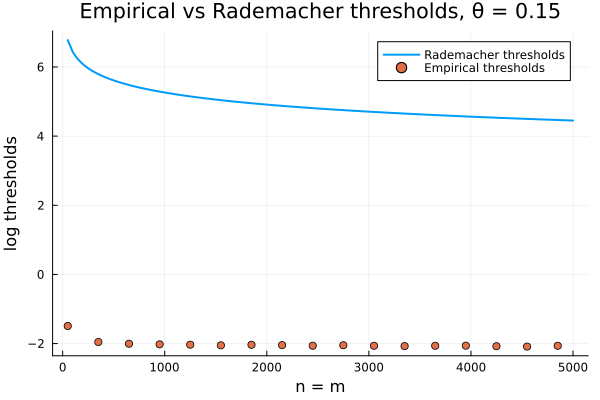
\includegraphics[width = \linewidth]{chapters/two-sample-testing/figures/ch4/emp_radem_plot_fixed_theta.png}
%     \end{subfigure}
%     \begin{subfigure}{0.32\textwidth}
%         \centering
%         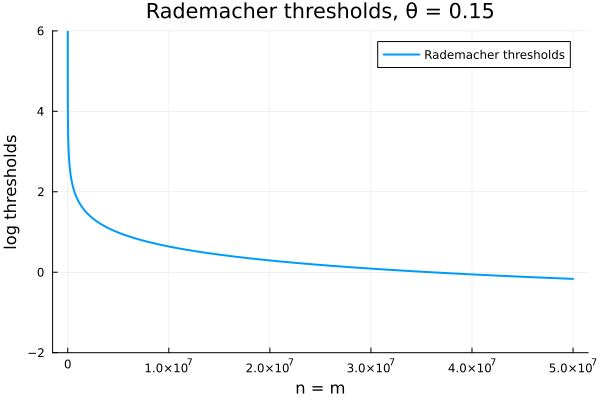
\includegraphics[width = \linewidth]{chapters/two-sample-testing/figures/ch4/radem_plot_vary_theta.png}
%     \end{subfigure}
%     \caption{}
%     \label{fig:radem_threshold_plots}
% \end{figure}

% summary: uniform, nonparametric thresholds via Rademacher complexity, HIPM yields faster rates than WoW,thresholds are overly conservative in practice.



